\section{Editor}
\label{sec:editor}
%TODO: May need newpage for layout reasons! Figures are booped up atm.
The editor, which allows the users to program their cells, is implemented with the following user interface, shown in \autoref{fig:editor_layout}

\begin{figure}[ht]
	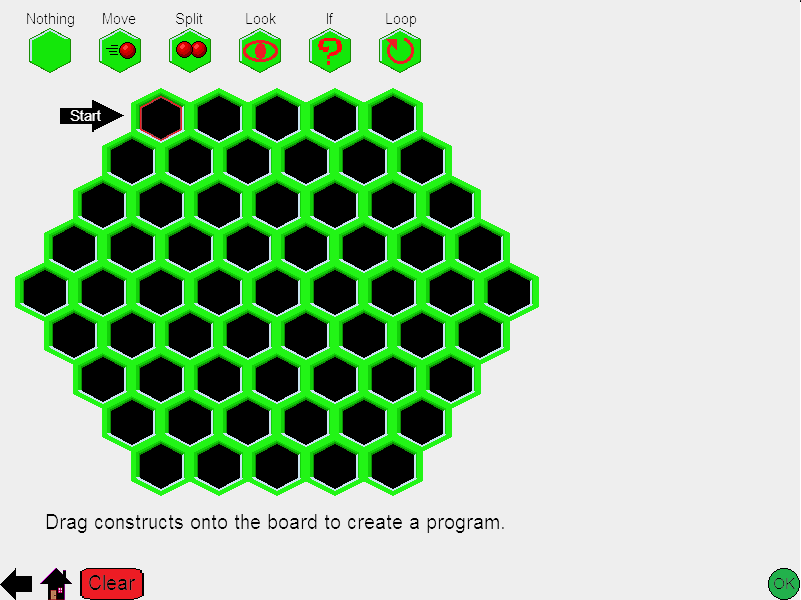
\includegraphics[width=0.75\textwidth]{img/editor_layout.png}
	\caption{Editor layout without form}
	\label{fig:editor_layout}
\end{figure}

The editor constructs are draggable and will snap into tiles on the board, if they are dropped over a tile.
Dragging a constructs creates a copy of the graphics to give the user a feeling of literally building a program.
Once the user drops the construct on the board, an HTML form/the details panel will pop up, allowing the user to customize the construct.
\autoref{fig:form_layout} shows the form for the loop construct:

\begin{figure}[ht]
	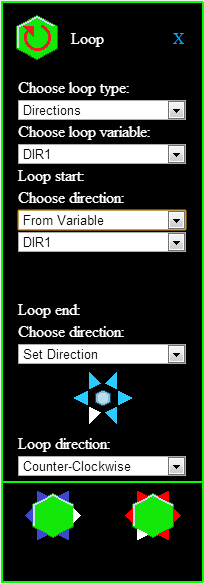
\includegraphics[scale=1]{img/editor_loop_form.png}
	\caption{Form layout for the loop construct}
	\label{fig:form_layout}
\end{figure}

When a tile is dragged the \texttt{Drag} class saves the type of instruction, while the construct is being moved.
Once it is dropped on the grid, the \texttt{Drag} class sends the coordinates of the drop and the instruction type to the \texttt{Editor} class, which then adds it in the \texttt{Program} class.\\

When the instruction is customized in the form, it is immediately updated in the \texttt{Program} class.
This means, that the user can input e.g. a number and, without pressing save or enter, close the form and the input automatically be saved.
It will then be there the next time the details panel is brought up.
Bringing up the details panel is done via clicking the tile on the grid.

The instructions are transferred as JS objects with a rather similar structure; below is the loop instruction shown as an example:

\begin{lstlisting}[language=javascript]
Instruction.loop = function()
{
	return {
		'type': 'loop',

		'expr_type': 'DIR',
		'variable': 'DIR1',
		'start':
		{
			'source': 'explicit',
			'value': 'R'
		},
		'end':
		{
			'source': 'explicit',
			'value': 'DL'
		},
		'increment': 'DV_COUNTERCLOCKWISE',
		
		'continue': 'R',
		'divert': 'DL'
	};
};
\end{lstlisting}

All instructions have a type.
In this case, the type of the instruction is \verb|'loop'|, and a direction where the program will continue in.
Some instructions, such as \verb|if| and \verb|loop|, have two directions for the program to continue due to our implementation of their behavior.
In between the type and the continue directions is the customizable information for that type.
The only instruction, that does not have any customization in between type and continue, is nop.